\section{Introduction}

The black Sigatoka disease caused by the fungus \emph{Mycosphaerella
  fijiensis Morelet} is the major pathological problem of banana and
plantain crops in Central America, Panama, Colombia and Ecuador, as well as in
many parts of Africa and Asia \citep{MarinVargas1995}.

This disease attacks the plant leaves producing a rapid deterioration
of the leaf area, affects the growth and productivity of the plants
due to the impairment of the photosynthetic process, causes a
reduction in the quality of the fruit, and promotes premature
ripening of bunches, which is
the major cause of product losses associated with the black
Sigatoka. \figref{fig:diseasestages} shows three stages of
this disease.
	 
\begin{figure}[ht] 
\centering
\begin{tabular}{c@{\;}c@{\;}c}
  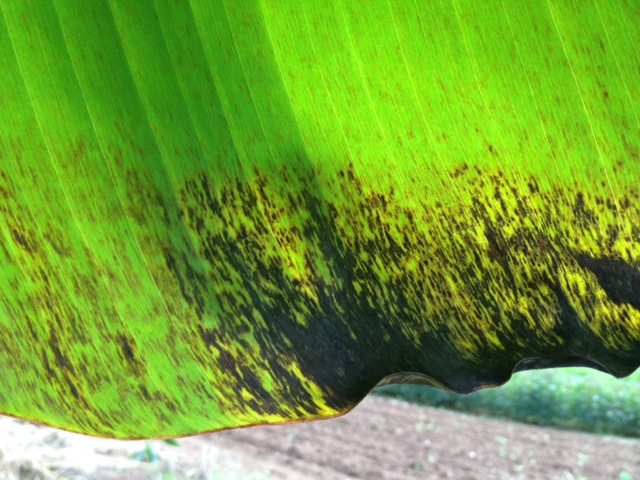
\includegraphics[width=.32\linewidth]{Roya_a} &
  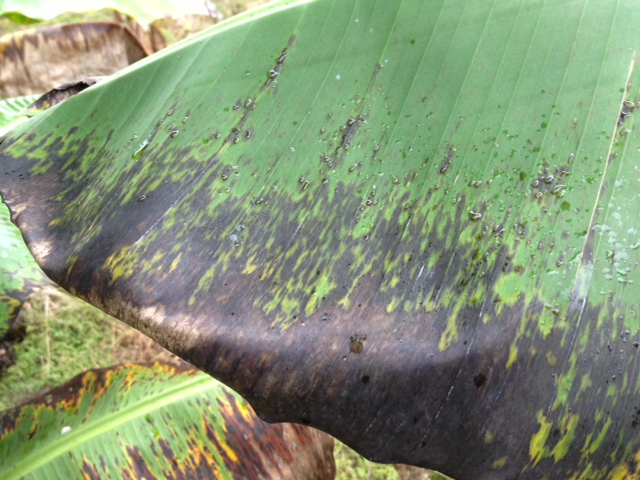
\includegraphics[width=.32\linewidth]{Roya_b} &
  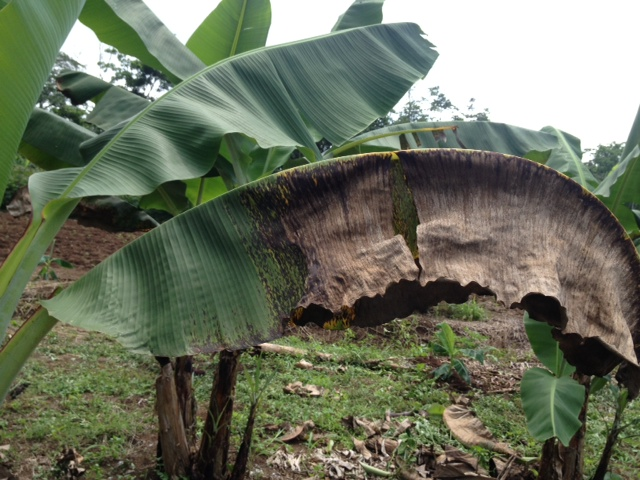
\includegraphics[width=.32\linewidth]{Roya_c} \\
  (a) & (b) & (c) 
\end{tabular}
\caption{Examples of three disease stages of the black Sigatoka. 
(a)~Initial stage. (b)~Intermediate stage, and (c)~Advanced stage.} 
\label{fig:diseasestages} 
\end{figure}

Phytopathological studies point out that precipitation, temperature,
relative humidity and wind are the main climatic variables that affect
the development of this disease \citep{MarinVargas1995}.

The climate has a major effect on the development of the black
Sigatoka.  Precipitation, temperature, relative humidity and wind are
the main climatic variables affecting the development of this disease
\citep{MarinVargas1995}.

The early warning system developed by Ganry and Meyer
\citep{ganry1972} and modified by Ganry and Laville \citep{ganry1983}
to control yellow Sigatoka in Cameroon, was later adapted by
Ternesien \citep{Ternesien1985} and Fouré \citep{foure1988} for the
black Sigatoka.

This bilogical warning system is based on weekly quantified
observations of the disease progression on young leaves of the plant,
according to Fouré's scale of the symptom stages.
%
Numeric coefficients are used to describe the degree of incidence and
the severity of the disease development.  These coefficients are used
to calculate two variables: gross sum and state of evolution.

The gross sum is based on the present disease progression stage and
the numeric coefficients, which increase with the progression of
the symptoms and the juvenility of the leaf.
%
The state of evolution is calculated using the gross sum and the
foliar emission period.
%
Although \todofn{threshold levels}% 
{No queda claro threshold levels sobre qué variables!?  Tampoco
  queda claro que quiere decir 'fluctuation' como medida de decisión}
%
were initially suggested as a guide to spray
schedules, the fluctuation of these two variables
was found to better define appropiate times to spray
\citep{Marinetal2003}.

In Costa Rica the black Sigatoka is frequently treated with
chemical fungicides.
%
Depending on the zone of production and the weather conditions,
45--55~cycles/year of fungicide applications are required to keep this
disease under control and to produce the expected fruit quality for the
international markets.
%
This represents a cost per hectare per year in the range between US\$1600 and
US\$2000; about 0.64--0.80 cents of the production costs for a
18.14\,kg box.
%
Overall, this represents 10\%--12\% of the total production costs.

The past and present rates of disease development can in principle be used
to predict its future behavior and to determine whether
a particular fungicide spray program will be able to effectively and
economically control the disease \citep{ChuangJeger1987} or not.

There are efforts to apply machine learning methods to support
decision-making in agriculture, including the control of crop
diseases. For example, \cite{Camargo2012} present an intelligent
system for the assessment of crop disorders, \cite{Huang2010}
introduce a plant virus identification method based on neural networks
with an evolutionary preprocessing stage, \cite{Kim2014} summarize in
their survey crop pests prediction methods using regression and
machine learning approaches, while \cite{Zhao2013} present an
intelligent agricultural forecasting system based on wireless sensor
networks.

In this work, we compare five machine learning techniques to predict
the development rate of the black Sigatoka disease: support vector
regression (SVR), echo state networks (ESN), ridge regression,
elastic-net regression and ordinary least squares linear regression.
%
\todofn{The main contribution of this work}%
{Definitivamente ese no es el aporte principal del artículo.  Cuando
  esté listo el resto hay que volver aquí.  Creo que va a ser algo
  como mostrar la relevancia de la etapa de preprocesamiento, o
  mostrar que a pesar de ser sistemas complejos, con variables
  caóticas, lo mejor en este caso son predictores lineales, o algo por
  el estilo.} %
% 
 is the selection of the best machine learning technique
to forecast the black Sigatoka development rate according to the
metric indicated below.

The outline of the paper is as follows: Section~\ref{sec:techs}
summarizes the machine learning techniques used in this research and
presents the main related works. In Section~\ref{sec:data} we present
the methodology used in this study and describe data used for its
verification.  The results and their discussion are presented in
section~\ref{sec:results}.  The Section~\ref{sec:concl} concludes this
article and presents lines for future works.

